\documentclass[11pt]{scrartcl}

\title{Märchen und andere Geschichten}
\author{Max Mustermann}
\date{\today{}, Berlin}

% \usepackage{ucs}
% \usepackage[utf8x]{inputenc}
% \usepackage[T1]{fontenc}

% Zeilenumbrüche der deutschen Sprache
% \usepackage[ngerman]{babel}

% Mathe-Stuff
\usepackage{amsmath,amssymb,amstext}

% zum Einfügen von Grafiken
\usepackage{graphicx}
 
 
 
\begin{document}

\maketitle
 
% Überschrift
\section{Einleitende Worte}
\label{sec:einleitende-worte} % optional

% \subsection
% \subsubsection 
% \paragraph{Einleitende Worte}
% \subparagraph

 
Finster war's, der Mond schien helle auf die grünbeschneite Flur, als
ein Wagen blitzesschnelle langsam um die runde Ecke fuhr. Drinnen
saßen stehend Leute schweigend ins Gespräch vertieft, als ein
totgeschossner Hase auf dem Wasser Schlittschuh lief und ein
blondgelockter Knabe mit kohlrabenschwarzem Haar auf die grüne Bank
sich setzte, die gelb angestrichen war. 


\subsubsection{Eine Aufzählung}

\begin{itemize}
  \item Alice im Wunderland
  \item Till Eulenspiegel
  \item Harry Potter
  \begin{itemize}
    \item Der Stein der Weisen
    \item Kammer des Schreckens
    \item Der Gefangene von Askaban
    \item Der Feuerkelch
    \item Der Orden des Phönix
  \end{itemize}
  \item Jim Knopf
\end{itemize}


\section{Mathematik}
\label{sec:mathematik}
 
\subsection{Unterstufe}
\label{sec:unterstufe}

\begin{equation*}
  a + 2 = c
\end{equation*}

\begin{equation*}
  a_{ij} - a_2 = 0
\end{equation*}

\begin{equation*}
  a^{ij} - a^2 = 0
\end{equation*}

\begin{equation*}
  \frac{1}{a} + \frac{1}{b} = \frac{a+b}{ab}
\end{equation*}

\begin{equation*}
  \sigma + \tau = \alpha
\end{equation*}
 
\subsection{Oberstufe} 
\label{sec:oberstufe}

\begin{equation}
  \label{eq:1}
  \left( \frac{a}{b} \right)' = \frac{a'b-ab'}{b^{2}}
\end{equation}

Es gilt die Invariante $b \neq 0$.

\begin{equation}
  \label{eq:2}
  \int\limits_{a}^{b} x^{2} \, dx = \frac{ b^{3} - a^{3} }{3}
\end{equation}

\begin{equation}
  \label{eq:3}
  c = \sqrt{ a^{2} + b^{2} }
\end{equation}



\section{Fortgeschrittene Anwendung}
\label{sec:fortg-anwend}
 
\subsection{Was macht Alice im Wunderland?}
\label{sec:was-macht-alice}

In Abschnitt \ref{sec:einleitende-worte} wurde ein Mädchen namens
Alice erwähnt. Was sie im Wunderland erlebt, kann in einem Buch
nachgelesen werden.
 
\subsection{Analyse}
\label{sec:analyse}

Die Gleichungen \eqref{eq:1} bis \eqref{eq:3} beherrschen wir bestens.
Alice, von der wir auf Seite \pageref{sec:einleitende-worte} gehört
haben, kennt diese Gleichungen wahrscheinlich nicht.

\begin{center}
  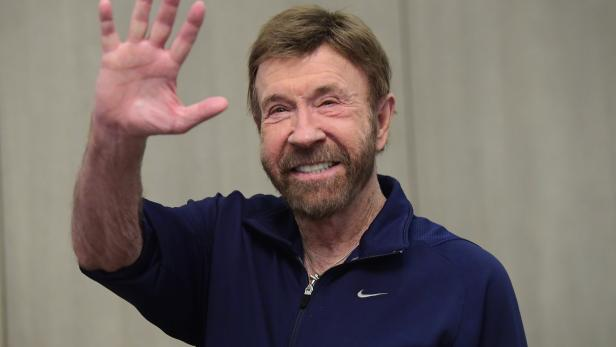
\includegraphics[width=0.1\textwidth]{chuck}
\end{center}
 
\end{document}